%%
%% Beuth Hochschule für Technik --  
%%
%% Kapitel 5 - 
%%
%%	

\newpage

[Perkowski]
\section{Simulation des Steuer- und Störverhaltens der Strecke} \label{Kapitel5}
Um zu überprüfen, ob sich unsere ermittelten Ergebnisse mit der realen Strecke gleichen, haben wir die Strecke samt Störung in Simulink modelliert (siehe Abbildung \ref{simustreckestor}).

\begin{figure}[h]
	\begin{center}
		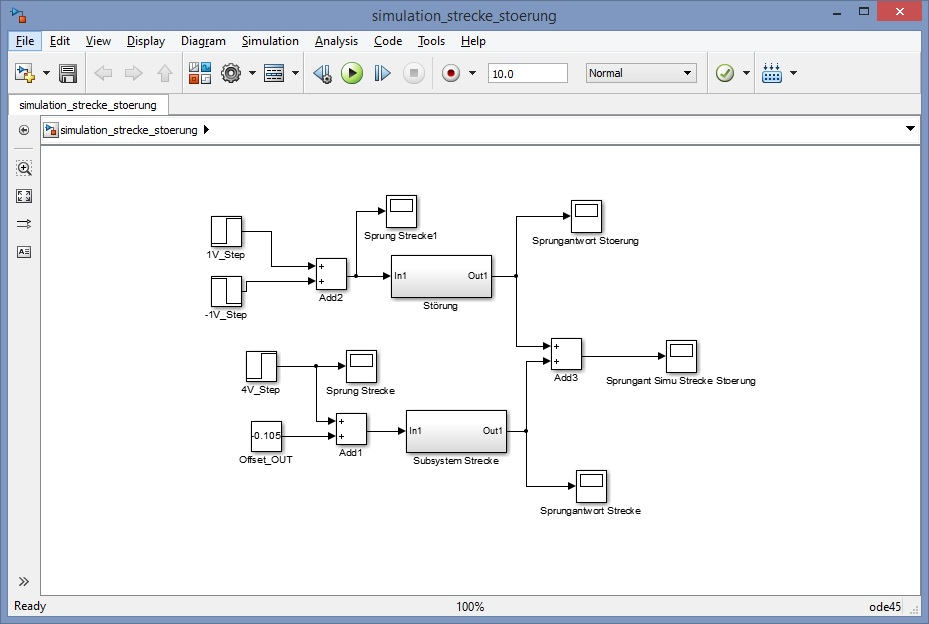
\includegraphics[scale=0.5]{simulink_simo_strecke_err.jpg}
		\caption{Simulink Modell der Strecke mit Störung}
       \label{simustreckestor}
	\end{center} 
\end{figure}


\begin{figure}[h]
	\begin{center}
		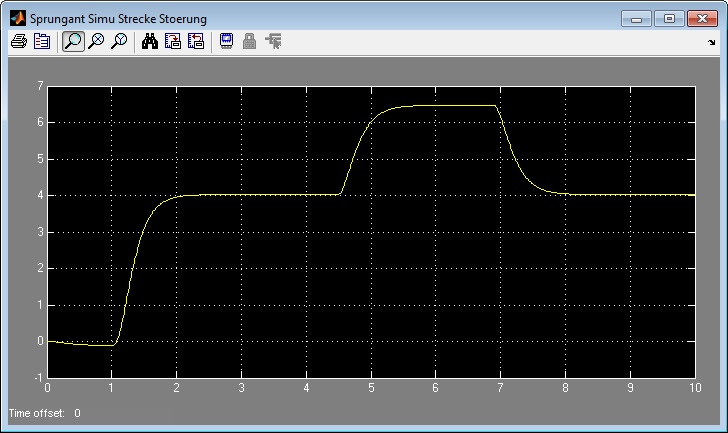
\includegraphics[scale=0.5]{simu_strecke_stoerung.jpg}
		\caption{Systemantwort des Modells der Strecke mit Störung}
       \label{plotsimustreckestor}
	\end{center} 
\end{figure}

Zu erkennen ist, dass sich unser Modell der realen Strecke gleicht (vergleiche Abbildung \ref{stoer} und \ref{plotsimustreckestor}).